% Chapter Template

\chapter{Numerical Investigation and Discussion} % Main chapter title

\label{Chapter6} % Change X to a consecutive number; for referencing this chapter elsewhere, use \ref{ChapterX}

This chapter will compare empirically the numerical and analytical methods presented for different types of contingent claims\footnote{The interested reader can see the implementation details in appendix \ref{AppendixD}}. The underlying model will be the black scholes model dating back to Black Scholes paper \parencite{B-S-Paper}\footnote{Assumption \ref{BS-Assumption}}, because it has closed form solutions for some European options and it is thoroughly researched.\\

The first section looks at the closed form solutions to the European options compared with the binomial lattice approch for pricing. The closed form solution gives a measure of how the binomial lattice model approximate European options. The binomial model is readily extended to American options, hence the section also gives a indication how the binomial model approximates the American options. The American put option is then investigated, where the different numerical methods considered are compared. The last types of options we look at are the exotic American options, where specially the bivariate contingent claim American put minimum will be considered. Futhermore will we compare the LSM and MLPs I pricing methods for American multivariate contingent claims with several underlyings. After the numerical investigation the model assumptions and choices in the thesis are discussed.


%----------------------------------------------------------------------------------------
%	SECTION 1
%----------------------------------------------------------------------------------------
\section{European Options}\label{EuroOption}
European options are simple in the sense, that they can only be exercised at maturity. Thoughout the previous chapters specially chapter \ref{Chapter2} and \ref{Chapter3} we have seen closed form solutions for the European call, call on max, call on min and geometric average options. The binomial lattice model presented is a numerical model to approximate European options and American options. The closed form solutions and the numerical lattice approch can be compared for European options, where a small deviation between methods for the European options indicates that the lattice approach gives reasonable prices for the American options.\\

The simplest case is the European call option, where we look how the CRR model and the MLPs II pricing model approximate the closed form solution. Table \ref{tab:EuroCall} shows empirically that the CRR model price prediction converge toward the price from the Black-Scholes call formula, which is inline with the theorectical result for the CRR model that it converges to the Black-Scholes model. The MLPs II model overprice the European call option, but it performs better for this example than the CRR with 10, 30 and 50 time-steps. The MLPs II is not practical for European call option, but it shows a relative close approximation, hence the increased speed for exotic options could be beneficial (TODO refer where you got numbers \href{https://www.rocq.inria.fr/mathfi/Premia/index.html}{Online Pricer}).\\

\begin{table}[th]
\caption{Comparision of accuracy for the European call option, where the inputs are K=40, $S_1(0)=40$, $\sigma_1=0.2$, T=1 and r=0.06.}
\label{tab:EuroCall}
\centering
\begin{tabular}{l l l}
\toprule
\textbf{Method} & \textbf{No. Steps} & \textbf{Price} \\
\midrule
CRR & 10 & 4.279\\
& 30 & 4.331\\
& 50 & 	4.342\\
& 100 & 4.350\\
& 200 & 4.354\\
& 500 & 4.357\\
& 1000 & 4.357\\
& 10000 & 4.358\\
MLPs II & & 4.370\\
Analytic form & & 4.358\\
\bottomrule\\
\end{tabular}
\end{table}

We see that the binomial model converge to the true price for the European call option. The natural extension of CRR model is the BEG model, where it is possible to price more exotic options. Section \ref{ExoticEuro} showed some closed form solution for exotic European options, hence we have a benchmark for the BEG in these special cases. We choose to look at computation time for European put minimum, which has a closed form solution\footnote{Equation \eqref{putMin} and \eqref{callMax}}. Closed form solutions make it easy to look at the trade-off between accuracy and computational cost for the BEG method. \\

\begin{table}[th]
\caption{Comparision of speed and accuracy for a European put min option, where the inputs are K=40, $S_1(0)=S_2(0)=40$, $\sigma_1=0.2, \sigma_2=0.3$, T=1, $\rho=0.5$  and r=0.06. Note ms is shorthand for millisecond}
\label{tab:TradeOffEuroMin}
\centering
\begin{tabular}{l l l l}
\toprule
\textbf{Method} & \textbf{No. Steps} & \textbf{Price} & \textbf{Time: min:sec.ms} \\
\midrule
BEG & 10 & 4.248 & 0:00.003\\
& 50 & 4.341 & 0:00:097\\
& 100 & 4.352 & 0:00.591\\
& 200 & 4.358 & 0:04.121\\
& 500 & 4.361 & 0:59.337\\
& 1000 & 4.362 & 9:34.164\\
Analytic form & & 4.363 & \\
\bottomrule\\
\end{tabular}
\end{table}
Tabel \ref{tab:TradeOffEuroMin} shows that the algorithm accuracy increases with the number of equidistant time-steps, but the computational speed dramatically slows down for high number of step, hence the computational cost become a factor to consider for more exotic options\footnote{Note that our implementation is written in python, hence room for improvement of code in terms of computational efficiency}. The BEG method accuracy is also tested on the European call minimum and European call maximum for 100 time-steps, where the BEG method is within 0.13 of the analytic solution (table \ref{tab:PriceEuropean}).\\
\begin{table}[th]
\caption{Valuation of bivariate contigent claims with K=40, $S_1(0)=S_2(0)=40$, $\sigma_1=0.2, \sigma_2=0.3$, T=1, $\rho=0.5$  and r=0.06.}
\label{tab:PriceEuropean}
\centering
\begin{tabular}{l l l l}
\toprule
\textbf{Derivative type} & \textbf{Method} & \textbf{No. Steps} & \textbf{Price} \\
\midrule
European Call Minimum & BEG & 100 & 2.475\\
& Analytic form & & 2.483\\
European Call Maximum & BEG & 100 & 7.787\\
& Analytic form & & 7.800\\
\bottomrule\\
\end{tabular}
\end{table}
 
The above tables shows that the binomial model pricing model can be used for both univariate and bivariate European contigent claims. The binomial models accuracy are high for European options, hence we expect a similar good approximatation for the American option. The CRR for univariate and BEG for bivariate contingent claims will be used as a benchmark for the American options, where we investigate LSM, MLPs I and MLPs II pricing methods. Note that the BEG is not practical for pricing multivariate contingent claims with many underlyings, because the possible states for the stochastic process increased exponentially. Therefore the bivariate case is important for comparision of the pricing methods.

\section{American Put Option}
The American put option has no analytically solution, hence numerical methods are required. We present and compare the results for the LSM, MLPs I and MLPs II pricing methods compared to the CRR model.\\

The LSM and MLPs I pricing method are almost identical, exept the MLPs tries to utilize deep learning to regress the expected continuation value. We have seen both methods converge to the optimal value process, hence we except numerically that by increasing the computational burden we approach the true price. To compare the two methods we simulate $10^5$ paths for the stock under the assumption that the future price of the stock is lognormal. The LSM and MLPs I pricing methods are used on the same simulated paths. The CRR and MLPs II\footnote{Note that we talk about the model after training} are not random in the sense that the output is deterministic, because both methods do not involve Monte Carlo simulation. For the LSM and MLPs I we assume 50 equidistant exercise dates for each year, where for the CRR we use 1000 equidistant time-step for the stock.  \\

The MLPs I require us to set some hyperparameters, where we choose the learning rate $\eta=0.001$, batch size of 512 and the Adam optimization algprithm. The architecture is a MLPs with three layers, where the hidden layers are with 40 neurons. The activation function is set to Leaky ReLU with 0.3 negative slope. The choices are partly inspired by the work by \parencite{Lelong19} and empirical testing. The regression in the LSM is done with a polynomial regression of degree 10. Remember the MLPs II is trained with the same hyperparameters as for the European call option.\\

\begin{table}[th]
\caption{Valuation of American put option with K=40 and r=0.06.}
\label{tab:AmericanPut}
\centering
\begin{tabular}{l l l l l l l }
\toprule
\textbf{Spot} & \textbf{$\sigma$} & \textbf{T} & \textbf{CRR} & \textbf{LSM} & \textbf{MLPs I} & \textbf{MLPs II} \\
\midrule
36 & 0.2 & 1 & 4.487 & 4.481 & 4.364 & 4.584\\
36 & 0.2 & 2 & 4.848 & 4.846 & 4.747 & 4.649\\
36 & 0.4 & 1 & 7.109 & 7.118 & 6.919 & 7.090\\
36 & 0.4 & 2 & 8.508 & 8.514 & 8.215 & 8.487\\
38 & 0.2 & 1 & 3.257 & 3.258 & 3.217 & 3.094\\
38 & 0.2 & 2 & 3.751 & 3.748 & 3.681 & 3.638\\
38 & 0.4 & 1 & 6.154 & 6.157 & 6.075 & 6.172\\
38 & 0.4 & 2 & 7.675 & 7.695 & 7.359 & 7.605\\
40 & 0.2 & 1 & 2.319 & 2.317 & 2.292 & 2.114\\
40 & 0.2 & 2 & 2.900 & 2.896 & 2.823 & 2.779\\
40 & 0.4 & 1 & 5.318 & 5.329 & 5.180 & 5.274\\
40 & 0.4 & 2 & 6.923 & 6.934 & 6.750 & 6.839\\
42 & 0.2 & 1 & 1.621 & 1.623 & 1.599 & 1.494\\
42 & 0.2 & 2 & 2.217 & 2.224 & 2.183 & 2.167\\
42 & 0.4 & 1 & 4.588 & 4.600 & 4.538 & 4.548\\
42 & 0.4 & 2 & 6.250 & 6.269 & 6.111 & 6.197\\
44 & 0.2 & 1 & 1.113 & 1.119 & 1.094 & 1.000\\
44 & 0.2 & 2 & 1.694 & 1.700 & 1.653 & 1.678\\
44 & 0.4 & 1 & 3.954 & 3.959 & 3.931 & 3.949\\
44 & 0.4 & 2 & 5.647 & 5.669 & 5.524 & 5.649\\
\bottomrule\\
\end{tabular}
\end{table}

Table \ref{tab:AmericanPut} shows that the MLPs I always predict a lower price than the LSM, hence for our numerical study the LSM seems to be better than the MLPs I in terms of approximatung the true price. The reference is the CRR model, which is a deterministisk method. The MLPs II trained with the CRR model shows high variability form the CRR predicted price compared to LSM. The total deviation in absolute distance for the MLPs II is 1.56, where LSM deviation is 0.157 for the above table containing 20 prices with different unique input parameters combinations. The MLPs II is though better in total absolute deviation compared to the MLPs I which has a total absolute deviation of 2.078. This indicates that the MLPs II at this stage of development is preferred over the MLPs I in terms of speed and accuracy. The MLPs I and LSM has some uncertainty from the Monte Carlo simulation, but with $10^5$ paths the standard error of the means are 0.0019 and 0.0214. The standard error\footnote{Sometimes written in short form SE} of the means are calculated by 100 samples\footnote{Denoted with n in the formulas} for the input parameters T=1,$\sigma=0.4$, $r=0.06$, $S(0)=36$, $K=40$. The empirical distribution mean is calculated by
$$\bar{x}= \frac{1}{n}\sum_{i=1}^{n} x_i$$
and the standard error of the mean
$$\sigma_{\bar{x}}= \frac{\sigma}{\sqrt{n}} \quad where \ \sigma=\sqrt{\frac{1}{n-1}\sum_{i=1}^{n} (x_i-\bar{x})}$$
 
The histogram (figure \ref{fig:histLSMMLPsI}) shows the variation in the estimates where the CRR price is the dashed black line. The histogram illustates the higher standard error for the MLPs I and a center of the distribution\footnote{Sample mean is 6.9048} lower than the CRR price\footnote{CRR price is 7.1094}. The LSM on the other hand has less variablity and the center\footnote{Sample mean is 7.1074} is around the CRR price, hence in term of numerical stability, computational speed and accuracy the LSM is superior for the American put. The reason to the numerical instability for the MLPs I is that the optimization algorithm is random on each run compared to the linear model\footnote{E.g. polynomial regression}.\\

\begin{figure}[th]
\centering
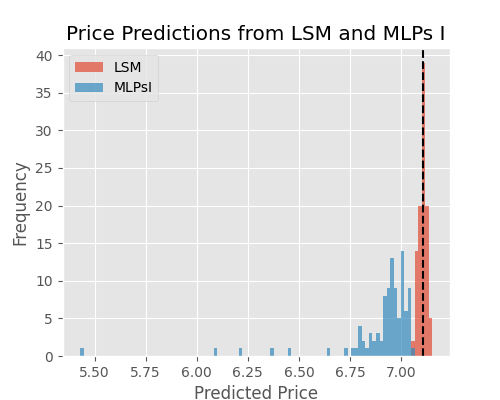
\includegraphics{Figures/histLSMMLPsI.png}
\decoRule
\caption[Histogram Price Predictions]{Predicted prices for American put option with LSM and MLPs. Parameters are T=1, $\sigma=0.4$, $r=0.06$, $S(0)=36$, $K=40$. Note CRR price is the dashed black line.}
\label{fig:histLSMMLPsI}
\end{figure}

Improvements of MLPs I is needed in order for the method to challenge the existing LSM both in terms of speed and accuracy for low dimensional problem. Possible improvement of the MLPs I could be conducted by a large hyperparameter tuning study. The earlier hyperparameter tuning methods could be applied, but more advanced methods could also be considered such as Bayesian hyperparameter tuning. The issue with hyperparameter tuning is that it is computational expensive. For the MLPs I the hyperparameter tuning need to be searched at every decision point. Another type of network could also be considered e.g. recurrent neural network. The inferior results from the MLPs I to the LSM shows that some work need still to be done. We choose not to consider MLPs I for the next section exotic American option.\\

The conclusion for the American put is that the classical methods are preferred over the MLPs pricing models.

\section{Exotic American Options}
There is many exotic american options to consider, but we choose to focus on the bivariate American put minimum option, because MLPs II is trained to predict prices on this specific option. The another advantage is that we have the deterministic method BEG to the bivariate contingent claim, hence the LSM and MLPs II can easy be compared both for accuray and speed.\\

First we need to decide how many time-steps we use for the BEG method. By looking at table \ref{tab:TradeOffAmerMin} is clear that the computational time is vary dependent on how many time-steps we choose. We know from the discussion in section \ref{EuroOption} that the accuracy increases by increasing the number of time-steps. Weighting the computational cost and accuracy we choose use a the BEG method as reference price with 500 time-steps. Note that when we generated the labels for the MLPs II pricing method we used 100 equidistant time-steps. The reason to use 100 time-steps is that we simulated 300.000 datapoints, which is a computational heavy task. We could have chosen more time-steps for a increased accuracy for the true price, but we judged the cost higher in terms of computational time than the benefits\footnote{It might be more beneficial to sample more data points than using a higher number of time-steps}.\\

\begin{table}[th]
\caption{Comparision of speed for the American put mininimum option, where the inputs are K=40, $S_1(0)=S_2(0)=40$, $\sigma_1=0.2, \sigma_2=0.3$, T=1, $\rho=0.5$  and r=0.06. Note ms is shorthand for millisecond}
\label{tab:TradeOffAmerMin}
\centering
\begin{tabular}{l l l l}
\toprule
\textbf{Method} & \textbf{No. Steps} & \textbf{Price} & \textbf{Time: min:sec.ms} \\
\midrule
BEG & 10 & 4.524 & 00:00.006\\
& 50 & 4.594 & 00:00.250\\
& 100 & 4.602 & 00:01.837\\
& 200 & 4.605 & 00:14.025\\
& 500 & 4.608 & 03:35.039\\
& 1000 & 4.609 & 28:32.584\\
\bottomrule\\
\end{tabular}
\end{table}

Note the price for the American put minimm (table \ref{tab:TradeOffAmerMin}) is greater than the the European put minimum (table \ref{tab:TradeOffEuroMin}). The another clear thing is that the computational time increases for the American option, because we have to compare intrinsic value and expected continuation value at each node. Both results are good sanity checks.\\

For visualization we plot the BEG, LSM and MLPs II for varying spots with fixed K=40, $\sigma_1=0.2$, $\sigma_2=0.3$, T=1, $\rho=0.5$  and r=0.06


\begin{table}[th]
\caption{Valuation of multivariate contigent claims with two underlyings with K=40, $S_1(0)=S_2(0)=40$, $\sigma_1=0.2, \sigma_2=0.3$, T=1, $\rho=0.5$  and r=0.06.}
\label{tab:PriceAmericanPut}
\centering
\begin{tabular}{l l l l}
\toprule
\textbf{Derivative type} & \textbf{Method} & \textbf{No. Steps} & \textbf{Price} \\
\midrule
\bottomrule\\
\end{tabular}
\end{table}





%----------------------------------------------------------------------------------------
%	SECTION 2
%----------------------------------------------------------------------------------------
Universal approximate theorem

The results will vary for each time running the algorithm given the stochastic nature in optimization and in sampling.


To compare the results by 


\parencite{liaw2018tune}

\section{Black Scholes Model}
In the B-S setup in section \ref{classicBS} we assume constant volatility, which is not realistic in terms of the known fact that volatility skew for equity options (p. 458 \parencite{Hull}).

The underlying risky equity assets is assumed in black scholes theory to evolve with a GBM, where the distribution of possible stock prices at the end of any interval is lognormal. Other models could have been considered e.g. the Bachelor model, where the differences in time for a stock are normal distributed. 
\begin{equation*}
dS_i=\sigma_i dW_i
\end{equation*}
This assumption would simplify the pricing problem of arithmetic basket options, because the problem is essentially one dimensionel like in the case with the geometric basket option for the black scholes model (section \ref{GeoBasket}). A disadvantage with the bachelier model is it can lead to negative stock values, which is not realistic. The Black-Scholes model has some drawbacks where you can question that is the probability distribution of asset prices really lognormal. \\

Empirical real data from markets has not constant volatility, but the volatility depends both on the maturity and strike, hence the investors talks about volatility shew or volatility smiles (chapter 20 \parencite{Hull}). The reason why equity options have shew in the volatility term structure is that investors are more concerned with falling stock prices than rising prices, hence the volatility are instantaneously negative correlated with the stock price. To overcome the issue about assuming constant volatility a model with stochastic variance can be considered. The model becomes more complex with a extra stochastic variable where for simplicity we consider the two factor Heston model. The basic model is given by the stock follow the SDE:
$$dS(t)=\alpha S(t) dt + \sqrt{V(t)} S(t) dW_S(t)$$
And the stochastic variance process $V(t)$ is the solution to the SDE:
$$dV(t)=a(\theta - V(t))dt + \epsilon \sqrt{V(t)} dW_V(t) \quad where a>0,\theta>0, \epsilon>0 \ and \ V(0)>0$$
Where $W_S(t)$ and $W_V(t)$ have correlation $\rho$. The interpretation of the constants are $\theta$ is long run average price variance, a is the rate which $V(t)$ reverts to $\theta$ and $\epsilon$ is the volatility of the volatility. The implication of $\epsilon$ is that $V(t)$ is more volatile when volatility is high and correlation between the stock and variance process reveals the negative correlation. The negative correlation between the two processes display the real market phenomenon of volatility shew for equity options, hence by assuming stochastic volatility the Heston model overcomes the issue with volatility shew.\\

Other models for describing the stochastic underlying process could be "Constant Elasticity of Variance model", "Merton's Mixed Jump-Diffusion Model", "Variance-Gamma Model"

Another underlying would could be the heston model

pay transaction costs and taxe

Options can be interpreted as corporate securities

credit risk and Mertons model

%----------------------------------------------------------------------------------------
%	SECTION 1
%----------------------------------------------------------------------------------------

%-----------------------------------
%	SUBSECTION 1
%-----------------------------------
\subsection{Neural Networks Vs. Linear Model}
Remember that neural network does not have curse of dimensionality, hence the method compared to the linear model has advantages when considering multivariate contingent claims.

%-----------------------------------
%	SUBSECTION 2
%-----------------------------------

\subsection{Subsection 2}
Computational time scales exponentially for PDE methods with the number of underlyings and the same goes for the binomial lattice approach, because both methods use dynamic programming. For the monte carlo methods the computational time only scales linear with the number of underlyings, where a smart method is needed for calculating stopping times.

Pricing options with early exercise decisions is not a issue with backward pricing methods.

%----------------------------------------------------------------------------------------
%	SECTION 2
%----------------------------------------------------------------------------------------

\section{Main Section 2}
\parencite{liaw2018tune}
\parencite{FergusonRyan2018}

Methods cannot be compared due to lack of code efficientcy. This is something that can be optimized. 

risk management find deltas.


    Pricing of Interest Rate Derivatives
    Pricing of Credit Risk Derivatives
    Pricing and Hedging of Equity Derivatives in Black-Scholes and Heston models
    Pricing and Hedging of Equity Derivatives in Jump models
    Calibration in Jump models
    
    but e.g. the LSM regression does not scale well for high dimensional rainbow options



    Antithetic variates and;
    Control variates.


"By its nature, simulation is a promising alternative to traditional finite difference and binomial techniques and has many advantages as a framework for valuing, risk managing, and optimally exercising American options. For example, simulation is readily applied when the value of the option depends on multiple factors."


Inpractice, lots of techniques are used to reduce the variance:
antithetic variables 
control variates
stratified sampling
importance sampling
quasi Monte Carlo methods